\chapter{Introduction à la Cryptographie}
\section{Principes généraux et termes}
\subsection{Points importants}
\subsubsection{Premier point}


% List
\begin{itemize}
	\item fonction de hachage,
	\item cryptographie symétrique,
	\item cryptographie asymétrique,
	\item infrastructures à clé publique (certificats).
\end{itemize}

% Figure with caption and label
\begin{figure}[h]
\centering
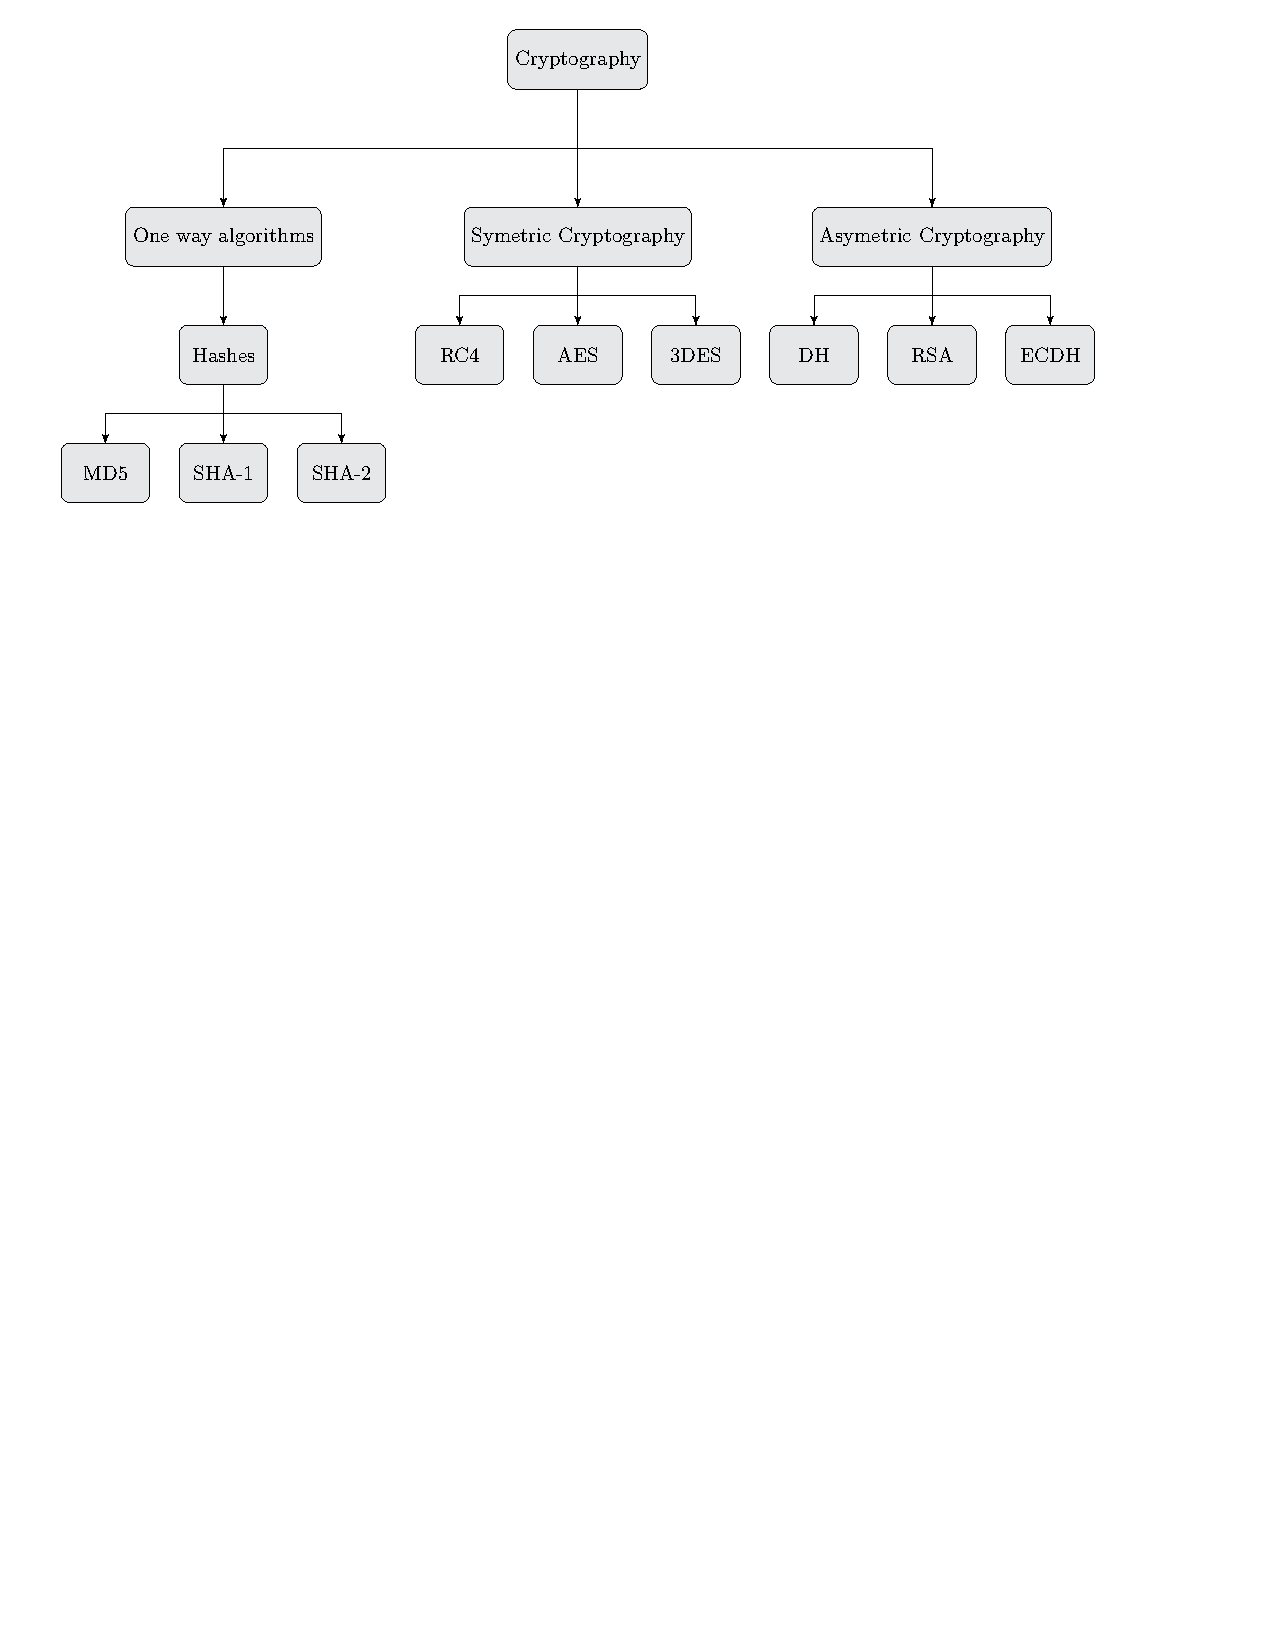
\includegraphics[trim= 0cm 19cm 3cm 0, clip,width=0.8\textwidth]{../figures/flowcharts/crypto_types.pdf}
\caption[Algorithmes de cryptographie importants]{Algorithmes de cryptographie importants}
\label{fig:crypto_algos}
\end{figure}
\FloatBarrier

% Table
\begin{table}[h]
	\vspace{0.5cm}
	% 3 columns + width of each column
		\begin{tabular}{|p{3cm}|p{4cm}|p{9cm}|}
		\hline
		%First line + bold horizontal line
		Nom & Taille du hash & Remarque \\ \Xhline{5\arrayrulewidth}
		MD5 & 128 bits  &  Déprécié \\ \hline
		SHA-1 & 160 bits & Déprécié par certains organismes (BSI\footnotemark[1], etc)  \\ \hline
		SHA-2 & 256 / 384 / 512 bits, dépend de la version utilisée & Recommandé \\ \hline
		\end{tabular}
	\caption{Caractéristiques des trois familles de fonctions de hachage}
	\label{hash_caracteristics}
\end{table}


% Quote from bibliography
% Reference to figure
Tous ces concepts sont expliqués en détail dans le livre \cite{understanding_cryp} ou à la figure \ref{fig:crypto_algos}.

%New page
\clearpage
% \cleardoublepage

% To prevent figures to be placed too far away
% Often used just after a figure or at the end of a section / subsection ,...
\FloatBarrier

% Footnote
\footnotetext[1]{Bundesamt für Sicherheit in der Informationstechnik, Allemagne}

% Todo
\todo[inline]{TODO: Remove this illustration}

%Source code inclusion
\lstinputlisting[linerange={104-128}, caption={sample C code - sample.c}, label={lst:sample}]{../source_code/sample.c}
